\chapter{Baseline setup}

\section{Overview}

\begin{figure}[h]
	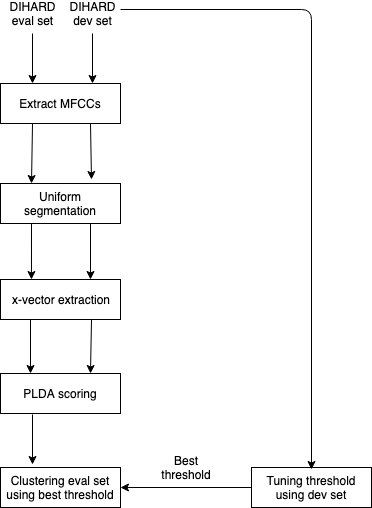
\includegraphics[width=9cm]{figures/baseline.png}
	\centering
	\caption{Block diagram of DIHARD diarization baseline.}
	\label{fig:fig-baseline}
\end{figure}

There are three software baselines provided by the DIHARD II organizers, each for the parts of speech enhancement, speech activity detection and diarization. The speech enhancement baseline and the speech activity detection are meant to be used together in the case of system-generated SAD (tracks 2 and 4), but since we only work with reference SAD, we do not need them. Thus we will only describe the diarization baseline in the following sections.

The diarization baseline is based on the best performing submission \cite{sell2018diarization} from John Hopkins University (JHU) in the previous year's DIHARD challenge (DIHARD I). There are 4 Kaldi recipes, each for an evaluation track, but we will focus only on the recipe for Track 1 since we only work with single channel audio and reference speech segmentation.

\section{Baseline directory structure}
The baseline repository is localted at \ttvar{https://github.com/iiscleap/DIHARD_2019_baseline_alltracks} and has the following directory structure. Some of the irrrelevant files have been removed.

\begin{verbatim}
DIHARD_2019_baseline_alltracks/
|-- data
|   |-- final.raw
|   |-- max_chunk_size
|   |-- min_chunk_size
|   |-- plda_track1
|   |-- plda_track2
|   |-- plda_track3
|   |-- plda_track4
|-- README.md
|-- recipes
|   |-- track1
|   |-- track2
|   |-- track2_den
|   |-- track3
|   |-- track4
|   `-- track4_den
|-- scripts
|   |-- alltracksrun.sh
|   |-- flac_to_wav.sh
|   |-- make_data_dir.py
|   |-- md_eval.pl
|   |-- prepare_feats.sh
|   |-- prep_eg_dir.sh
|   `-- split_rttm.py
`-- tools
    |-- env.sh
    |-- install_dscore.sh
    |-- install_kaldi.sh
}
\end{verbatim}

The \ttvar{data} directory has pre-trained models (in Kaldi binary format) and some configuration parameters. \ttvar{final.raw} is the DNN x-vector extractor, and the \ttvar{plda_*} files are the PLDA backends trained for the 4 tracks. The \ttvar{recipes} directory has the \ttvar{run.sh} files for all 4 recipes, we only care about \ttvar{track1}. The \ttvar{scripts} directory has extra scripts that are needed on top of the \ttvar{egs/dihard_2018} Kaldi recipe - \ttvar{alltracksrun.sh} is the main diarization script, \ttvar{make_data_dir.py} makes the Kaldi data directory from the DIHARD datasets (creating the files wav.scp, segments, utt2spk), \ttvar{prep_eg_dir.sh} copies the extra files from this repository to the \ttvar{egs/dihard_2018} directory, \ttvar{md_eval.pl} \cite{mdeval2006} is a diarization evaluation script that was developed by NIST, and others are self-explanatory. The \ttvar{tools} directory holds scripts to install Kaldi and dscore \cite{dscore}, which are installed in the same directory.

The baseline code modifies and reuses the \ttvar{egs/dihard_2018} recipe that was checked into Kaldi by the researchers at JHU. It does this by copying over new scripts and data that is needed to the \ttvar{egs/dihard_2018} directory, \ttvar{cd}'ing to that directory and running the recipe from there.

We modify and add scripts in this repository so we can easily run experiments with different parameters. The \ttvar{run.sh} script is modified to allow easily changing parameters to run different experiments.

\section{Initial segmentation}
The initial segmentation step is done by \ttvar{make_data_dir.py}. It deals with separating speech and non-speech segments from the recording files using the reference SAD.

This results in a bunch of segments which are known to be containing only speech. These are treated as ``utterances" in Kaldi terminology and act as keys in the \ttvar{utt2spk}, \ttvar{feats.scp} and \ttvar{segments} files. These files reside in two Kaldi ``data directories", one for each dev and eval.

\section{Features}
The baseline then extracts 30 dimensional MFCC features using a 25 ms window that shifts by 10 ms. It uses the standard \ttvar{steps/make_mfcc.sh} Kaldi script for this. The MFCC configuration used \ttvar{mfcc.conf} is given below.

\begin{verbatim}
--sample-frequency=16000
--frame-length=25 # the default is 25
--low-freq=20 # the default.
--high-freq=7600 # Nyquist (8k in this case).
--num-mel-bins=30
--num-ceps=30
--snip-edges=false
\end{verbatim}

Later, cepstral mean and variance normalization (CMVN) with a 3 second sliding window is applied using the \ttvar{apply-cmvn-sliding} Kaldi tool.

\section{Subsegmentation}
After MFCC extraction is done for the segments, the segments are uniformly divided into smaller 1.5 second subsegments with a 0.75 second overlap. This creates new Kaldi data directories (one each for dev and eval sets) with newer keys corresponding to each subsegment.

\section{Speaker representation}
The baseline extracts an 512-dimensional x-vectors from each subsegment. The DNN extractor \ttvar{final.raw} is trained on the datasets VoxCeleb I and II, along with added augmentation.

\section{Scoring}
For scoring two x-vectors, PLDA scores are used as a distance metric. The \ttvar{plda_track1} file is used which has been trained using x-vectors extracted from a random subset (size 128k) of the VoxCeleb dataset. To adapt the extracted x-vectors to the DIHARD domain, they are whitened with a whitening transform learned from the DIHARD development set. Each pair of x-vectors within a recording is then scored using the PLDA backend by reusing \ttvar{score_plda.sh} from \ttvar{egs/callhome_diarization}. These scores are stored in matrix form for each recording.

\section{Clustering}
The x-vectors are then clustered using agglomerative clustering and a parameter sweep is done on the dev set to find the threshold that maximises the DER on the dev set. This threshold is then used for clustering the x-vectors of the eval set. The \ttvar{agglomerative-cluster} Kaldi binary is used for clustering.

\section{Diarization output}
The clustering output is used to generate RTTMs using the script \ttvar{make_rttm.py} from \ttvar{egs/callhome_diarization}. The RTTMs give a flat segmentation of the recordings with no overlap. Since the x-vectors were extracted from segments that were overlapping, care needs to be taken when two adjacent segments are assigned to a different speaker. The script places the speaker boundary midway between the end of the first segment and the start of the second segment.

